\documentclass[12pt, a4paper]{article}

%%%%%%%%%%%%%%%紙張大小設定%%%%%%%%%%%%%%%
% \paperwidth=65cm
% \paperheight=160cm

%%%%%%%%%%%%%%%引入Package%%%%%%%%%%%%%%%
\usepackage[margin=1cm]{geometry} % 上下左右距離邊緣2cm
\usepackage{mathtools,amsthm,amssymb} % 引入 AMS 數學環境
\usepackage{yhmath}      % math symbol
\usepackage{graphicx}    % 圖形插入用
\usepackage{fontspec}    % 加這個就可以設定字體
\usepackage{type1cm}	 % 設定fontsize用
\usepackage{titlesec}   % 設定section等的字體
\usepackage{titling}    % 加強 title 功能
\usepackage{fancyhdr}   % 頁首頁尾
\usepackage{tabularx}   % 加強版 table
\usepackage[square, comma, numbers, super, sort&compress]{natbib}
% cite加強版
\usepackage[unicode, pdfborder={0 0 0}, bookmarksdepth=-1]{hyperref}
% ref加強版
\usepackage[usenames, dvipsnames]{color}  % 可以使用顏色
\usepackage[shortlabels, inline]{enumitem}  % 加強版enumerate
\usepackage{xpatch}

\graphicspath{ {images/} }
% \usepackage{tabto}      % tab
% \usepackage{soul}       % highlight
% \usepackage{ulem}       % 字加裝飾
\usepackage{wrapfig}     % 文繞圖
%\usepackage{lipsum}
% \usepackage{floatflt}    % 浮動 figure
\usepackage{float}       % 浮動環境
% \usepackage{caption}    % caption 增強
% \usepackage{subcaption}    % subfigures
% \usepackage{setspace}    % 控制空行
% \usepackage{mdframed}   % 可以加文字方框
% \usepackage{multicol}   % 多欄
% \usepackage[abbreviations]{siunitx} % SI unit
% \usepackage{dsfont}     % more mathbb

%%%%%%%%%%%%%%%%%%%TikZ%%%%%%%%%%%%%%%%%%%%%%
% \usepackage{tikz}
% \usepackage{circuitikz}

%%%%%%%%%%%%%%中文 Environment%%%%%%%%%%%%%%%
\usepackage[CheckSingle, CJKmath]{xeCJK}  % xelatex 中文
\usepackage{CJKulem}	% 中文字裝飾
\setCJKmainfont{Source Han Sans}
% 設定中文為系統上的字型,而英文不去更動,使用原TeX字型

% \XeTeXlinebreaklocale "zh"             %這兩行一定要加,中文才能自動換行
% \XeTeXlinebreakskip = 0pt plus 1pt     %這兩行一定要加,中文才能自動換行

%%%%%%%%%%%%%%%字體大小設定%%%%%%%%%%%%%%%
% \def\normalsize{\fontsize{10}{15}\selectfont}
% \def\large{\fontsize{40}{60}\selectfont}
% \def\Large{\fontsize{50}{75}\selectfont}
% \def\LARGE{\fontsize{90}{20}\selectfont}
% \def\huge{\fontsize{34}{51}\selectfont}
% \def\Huge{\fontsize{38}{57}\selectfont}

%%%%%%%%%%%%%%%Theme Input%%%%%%%%%%%%%%%%
% \input{themes/chapter/neat}
% \input{themes/env/problist}

%%%%%%%%%%%titlesec settings%%%%%%%%%%%%%%
% \titleformat{\chapter}{\bf\Huge}
            % {\arabic{section}}{0em}{}
% \titleformat{\section}{\centering\Large}
            % {\arabic{section}}{0em}{}
% \titleformat{\subsection}{\large}
            % {\arabic{subsection}}{0em}{}
% \titleformat{\subsubsection}{\bf\normalsize}
            % {\arabic{subsubsection}}{0em}{}
% \titleformat{command}[shape]{format}{label}
            % {編號與標題距離}{before}[after]

%%%%%%%%%%%%variable settings%%%%%%%%%%%%%%
% \numberwithin{equation}{section}
% \setcounter{secnumdepth}{4}  %章節標號深度
% \setcounter{tocdepth}{1}  %目錄深度
% \setcounter{section}{0}  %section 起始 counter
% \graphicspath{{images/}}  % 搜尋圖片目錄

%%%%%%%%%%%%%%%頁面設定%%%%%%%%%%%%%%%
\newcolumntype{C}[1]{>{\centering\arraybackslash}p{#1}}
\setlength{\headheight}{15pt}  %with titling
\setlength{\droptitle}{-2cm} %title 與上緣的間距
% \posttitle{\par\end{center}} % title 與內文的間距
\parindent=12pt %設定縮排的距離
% \parskip=1ex  %設定行距
% \pagestyle{empty}  % empty: 無頁碼
% \pagestyle{fancy}  % fancy: fancyhdr

% use with fancygdr
% \lhead{\leftmark}
% \chead{}
% \rhead{}
% \lfoot{}
% \cfoot{}
% \rfoot{\thepage}
% \renewcommand{\headrulewidth}{0.4pt}
% \renewcommand{\footrulewidth}{0.4pt}

% \fancypagestyle{firststyle}
% {
  % \fancyhf{}
  % \fancyfoot[C]{\footnotesize Page \thepage\ of \pageref{LastPage}}
  % \renewcommand{\headrule}{\rule{\textwidth}{\headrulewidth}}
% }

%%%%%%%%%%%%%%%重定義一些command%%%%%%%%%%%%%%%
\renewcommand{\contentsname}{目錄}  %設定目錄的標題名稱
\renewcommand{\refname}{參考資料}  %設定參考資料的標題名稱
\renewcommand{\abstractname}{\LARGE Abstract} %設定摘要的標題名稱

%%%%%%%%%%%%%%%特殊功能函數符號設定%%%%%%%%%%%%%%%
\DeclarePairedDelimiter{\abs}{\lvert}{\rvert}
\DeclarePairedDelimiter{\norm}{\lVert}{\rVert}
\DeclarePairedDelimiter{\inpd}{\langle}{\rangle} % inner product
\DeclarePairedDelimiter{\ceil}{\lceil}{\rceil}
\DeclarePairedDelimiter{\floor}{\lfloor}{\rfloor}
\DeclareMathOperator{\adj}{adj}
\DeclareMathOperator{\sech}{sech}
\DeclareMathOperator{\csch}{csch}
\DeclareMathOperator{\arcsec}{arcsec}
\DeclareMathOperator{\arccot}{arccot}
\DeclareMathOperator{\arccsc}{arccsc}
\DeclareMathOperator{\arccosh}{arccosh}
\DeclareMathOperator{\arcsinh}{arcsinh}
\DeclareMathOperator{\arctanh}{arctanh}
\DeclareMathOperator{\arcsech}{arcsech}
\DeclareMathOperator{\arccsch}{arccsch}
\DeclareMathOperator{\arccoth}{arccoth}
\newcommand{\np}[1]{\\[{#1}] \indent}
\newcommand{\transpose}[1]{{#1}^\mathrm{T}}
%%%% Geometry Symbol %%%%
\newcommand{\degree}{^\circ}
\newcommand{\Arc}[1]{\wideparen{{#1}}}
\newcommand{\Line}[1]{\overleftrightarrow{{#1}}}
\newcommand{\Ray}[1]{\overrightarrow{{#1}}}
\newcommand{\Segment}[1]{\overline{{#1}}}

%%%%%%%%%%%%%%%證明、結論、定義等等的環境%%%%%%%%%%%%%%%
\renewcommand{\proofname}{\bf 證明:} %修改Proof 標頭
\newtheoremstyle{mystyle}% 自定義Style
  {6pt}{15pt}%       上下間距
  {}%               內文字體
  {}%               縮排
  {\bf}%            標頭字體
  {.}%              標頭後標點
  {1em}%            內文與標頭距離
  {}%               Theorem head spec (can be left empty, meaning 'normal')

% 改用粗體,預設 remark style 是斜體
\theoremstyle{mystyle}	% 定理環境Style
\newtheorem{theorem}{定理}
\newtheorem{definition}{定義}
\newtheorem{formula}{公式}
\newtheorem{condition}{條件}
\newtheorem{supposition}{假設}
\newtheorem{conclusion}{結論}
\newtheorem{corollary}{推論}
\newtheorem{lemma}{引理}
\newtheorem{property}{性質}

\titlespacing*{\section} {0pt}{0ex}{0ex}

%%%%%%%%%%%%%%%Title%%%%%%%%%%%%%%%
\title{MLDS 2017 Spring HW2 - Seq2Seq \& Attention}
\author{B03901056 孫凡耕 B03901070 羅啟心\\
        B03901032 郭子生 B03901003 許晉嘉}
\date{\vspace{-5ex}}

\begin{document}
\maketitle 
\pagenumbering{gobble}% Remove page numbers (and reset to 1)
\thispagestyle{empty}
\section{Environment}
%\begin{enumerate}
  %\item 硬體資訊: \\
  \begin{table}[h]
  \centering
    \begin{tabular}{|C{4cm}|C{2.5cm}|C{3cm}|C{2.5cm}|C{3cm}|}
      \hline
      OS & CPU & CPU Memory & GPU & GPU Memory \\
      \hline
      \texttt{Arch linux 4.10} &
      \texttt{i7 3.6 GHz} &
      \texttt{32 GB} &
      \texttt{GTX 1080 Ti}  &
      \texttt{11 GB}  \\
      \hline
    \end{tabular}
  \end{table}
%\end{enumerate}
% End of Environment

\section{Model description}
\begin{enumerate}
\item Seq2Seq 模型:\\
典型的 encoder-decoder 的模型,也就是利用 LSTM 把不同長度的輸入,
轉化為固定大小的 state,然後將此 state 傳遞給另個 LSTM,並依序輸
出當前最佳解直到遇到 \texttt{<eos>} 爲止。\\
模型所使用的參數如下:
\begin{itemize}
  \item batch\_size = 145
  \item video and word embedding dimension: 4096
  \item layer\_num = 2
  \item rnn\_cell = LSTM with peephole
  \item hidden\_size = 256
  \item optimizer = adam
  \item dropout keep prob = 0.7
  \item with bidirectional rnn at encoder
  \item with attention (bahdanau)
  \item with scheduled sampling (linear decrease to 0.5)
\end{itemize}
\item S2VT 模型:\\
在 sequence to sequence 之外,我們也根據 paper 實作出了 S2VT 的模型。
不同於傳統 seq2seq 是由一層 encoder 和一層 decoder 所組成,S2VT 是由
兩個 LSTM cell 在時間軸上分成 encoding 和 decoding 的階段。影片在
encoding 階段每個 frame 做 embedding 至 500 維,作為第一個 LSTM 的輸入,
第一個 LSTM 的輸出和 \texttt{<pad>} 做 concat 之後即為二個 LSTM 在 encoding
階段的輸入;在 decoding 階段,第一個 LSTM 輸入不再是影片的 embedding,
而改為輸入 \texttt{<pad>} ,第一個 LSTM 的輸出和 embedded 的 word 做 concat
之後即為第二個 LSTM 的輸入。值得一提的是 decoding 階段要以輸出 \texttt{<bos>}
作為開頭,並以第二個 LSTM 輸出的 \texttt{<eos>} 當作結尾。模型參數如下:
\begin{itemize}
  \item batch\_size = 290
  \item video and word embedding dimension: 500
  \item rnn\_cell = LSTM with peephole
  \item hidden\_size = 1000
  \item optimizer = adam
  \item dropout keep prob = 0.7
\end{itemize}
\begin{figure}[!htb]
  \centering
  \minipage{1\textwidth}
  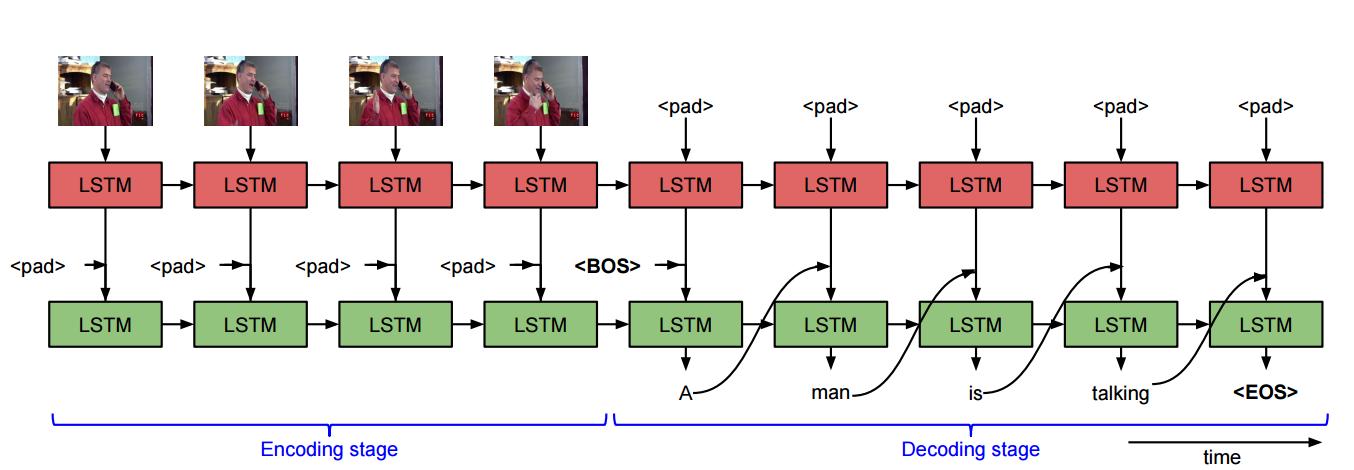
\includegraphics[scale=0.4]{s2vt.png}
  \caption{S2VT 模型架構}
  \label{fig:s2vt}
 \endminipage
\end{figure}

\end{enumerate}
% End of Model description

\section{Improvement}
我們在 seq2seq 的模型之中做了許多的 improvement,包含加上
attention、bidirectional、schedule sampling 等等。而在傳統的
seq2seq 模型之外,我們也根據 paper 嘗試使用 S2VT 作為本次作業的
improvement,並在 S2VT 上加了 schedule sampling 做更進一步的優化,
以及一些不同於 paper 在參數上的調整實驗。比較可惜的是在時間內我們並沒有在
S2VT 的模型中看到比 seq2seq 更好的結果,而最終 S2VT 模型在 bleu 分數表現上
最好的結果大約是 0.22 左右。
一些輸出的結果如下:
\begin{itemize}
  \item \texttt{a man is dumping pasta into a plate}
  \item \texttt{a man is playing the guitar on stage}
  \item \texttt{a person with a cleaver is slicing an onion}
\end{itemize}

\begin{enumerate}
\item Attention \\
  我們嘗試比較不同 Attention 以及使用 Attention 與否。從 Figure~\ref{fig:cmpat}
  中可以發現,當不使用 Attention 時,學習的過程十分緩慢,並且訓練的效果極差,幾乎
  無法有學習的效果。但加上 Attention 之後,學習的效果便十分顯著。而兩種 Attention
  的方式大致來說並沒有顯著的差異。
\item Bi-directional \\
  我們嘗試比較使用 Bi-directional 與否。並分爲使用 Attention 與否的兩種情況討論:
  \begin{itemize}
  \item 不使用 Attention\\
    從 Figure~\ref{fig:at0} 中可以看出,在不使用 Attention 的情況下,加上
    Bi-directional 時,學習的過程會比較緩慢,並且學習的效果並不會比較好。我們
    推論,這是由於不使用 Attention 時,由 Bi-directional 從後方 feedback 回來
    的資訊,對於當前的 cell 而言,就相當於雜訊一般。因此,不僅無法提升學習的效果
    ,反而會阻礙學習的過程,因此,在訓練上的學習效果便會比較差。
  \item 使用 Attention \\
    從 Figure~\ref{fig:at1} 及 Figure~\ref{fig:at2} 中可以看出,當使用 Attention 時,
    加上 Bi-directional 會加強學習的效果,這是由於有 Attention 的幫助下,能學習
    到 Bi-directional 回來的資訊以及前方資訊的關聯,進而提升訓練的成效。
  \end{itemize}
\item Scheduled Sampling \\
  從 Figure~\ref{fig:at0} 到 Figure~\ref{fig:at2} 中可以看出,使用 Scheduled Sampling
  會使 perplexity 的變化較爲動盪,但在這次的作業中,使用 Scheduled Sampling
  並沒有顯著的提升學習成效的現象。
\item Word embedding \\
  原先的模型中,我們對於任意一個單詞,是先隨機初始值來進行訓練,但事實上,我們
  應該是有辦法先對 caption 進行分析,來達成更好的訓練效果。因此,我們將 caption
  的單詞先蒐集起來,自己訓練出這些單詞的 word embedding,如此一來,就將變數改爲
  固定的 pretrained 值,而不是隨機的變數。另外,我們原先使從若干句 caption 中挑
  一句出來作爲訓練資料,其他句子便完全沒有運用到。如此一來,我們所看過的句子就
  只有一千多句。而現在我們預先訓練自己的 word embedding,便能利用到其他 caption
  所提供的語料資訊。
\item Black Magic \\
  原先的訓練資料是以 80 個 frame 的影片對應若干個 caption,而我們原先是將一個
  影片對應一個 caption 做訓練。而現在,我們可以將 80 個 frame 分爲五組不相交的
  16 個 frame 分別對應一個 caption,相對於分爲五個影片。由於訓練模型的結構,我們
  同樣可以以這組資料做訓練。而測試的時候,同樣以 80 個 frame 作爲輸入,如此訓練
  出來的效果,會比原先的結果來的較好。原先的 bleu score 大約 0.29,使用此方法後,
  bleu score 最高進步到 0.32。
\item from static to dynamic \\
  原始的 S2VT 我們使用 for 迴圈進行實作,然而這種做法會使得 model 在 tensorflow
  中被展開使得記憶體使用量過大,因此我們最後 S2VT 是用 tensorflow 當中的
  raw\_rnn 搭配 tensorflow 內建的 loop function 實作,如此便可避免記憶體使用量
  的問題。
  \begin{figure}[!htb]
    \centering
    \minipage{0.5\textwidth}
    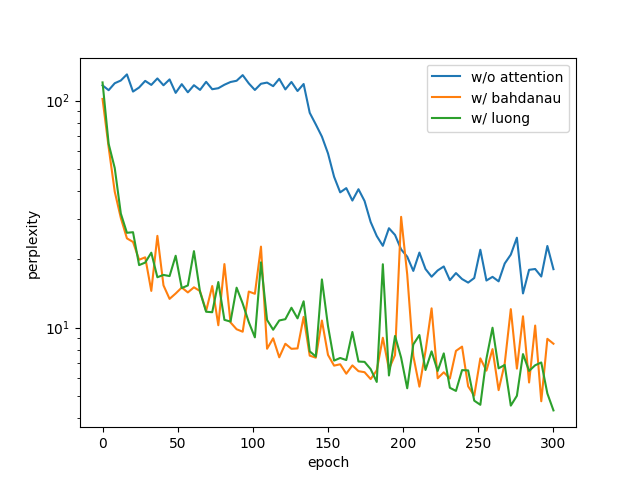
\includegraphics[scale=0.5]{cmp_at_perplex.png}
    \caption{不同 Attention 間之比較}
    \label{fig:cmpat}
   \endminipage
   \hfill
    \minipage{0.5\textwidth}
    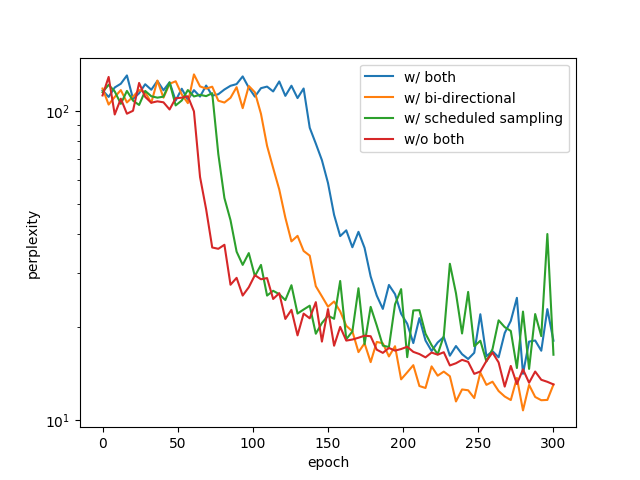
\includegraphics[scale=0.5]{at0.png}
    \caption{不使用 Attention}
    \label{fig:at0}
   \endminipage
   \hfill
    \minipage{0.5\textwidth}
    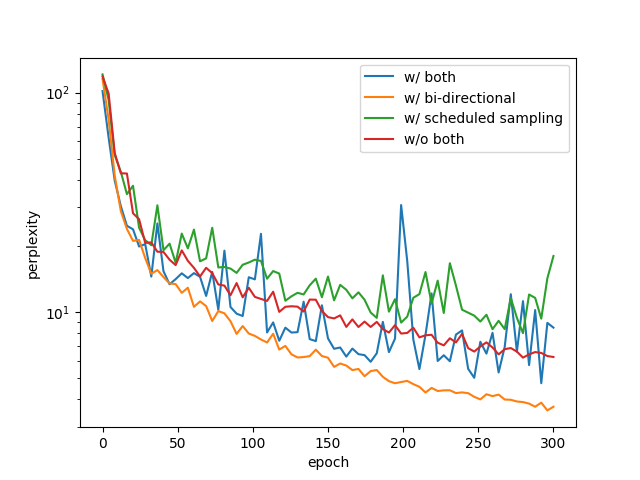
\includegraphics[scale=0.5]{at1.png}
    \caption{bahdanau Attention}
    \label{fig:at1}
   \endminipage
   \hfill
    \minipage{0.5\textwidth}
    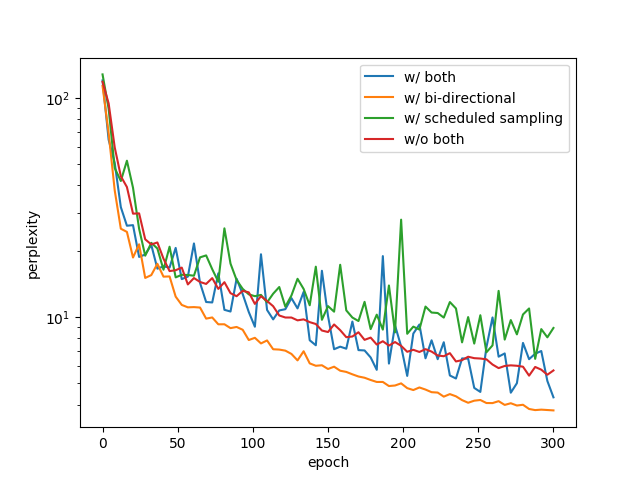
\includegraphics[scale=0.5]{at2.png}
    \caption{luong Attention}
    \label{fig:at2}
   \endminipage
  \end{figure}
\end{enumerate}
% End of Improvement

\section{Experiment}
\begin{enumerate}
\item  對於 S2VT 模型,我們首先對於原始 Paper 的 Model 進行重現,接著便在參數以及
模型上進行嘗試與調整。在 Cell 種類的改變下,如 Figure~\ref{fig:jason} 所示,
可以發現在 training 的過程中的確有 GRU、快於 BasicLSTM、又快於 FullLSTM 的
趨勢,但整體表現上還是 FullLSTM(含有 peephole )的表現較佳。另外我們對於
每個影片只取出一個 caption 為該影片中所有 caption 長度中位數的做 training,
並從影片的 80 個 frame 中每 1, 4, 8, 10 的 frame 取一張做為 input,可以發現
當取出一個 caption 以及每 4 個 frame 取出一張會在 bleu 分數上稍有進步,但並
沒有太大的不同。此外我們也在 S2VT 的模型中加入 schedule sampling,但 bleu 的
分數反而下降到 0.194 左右,並沒有比原先的 S2VT 更為進步。
\item 從 Figure~\ref{fig:score} 中可以看出,在剛開始的時候(大約 200 epoch 時),
  bleu score 就已經很高,超過 baseline 達到 0.28 左右,但事實上,每次所預測出的句子
  都是 \texttt{A man is playing a guitar},所以實際上並沒有學習的效果。雖然隨着
  perplexity 的下降,bleu score 也跟着下降,但實際上所學習出來的句子更爲精準。
  但因爲模型所預測出的句子,有時候無法切題,因此 bleu score 相對來說,反而略微下降。
  當 perplexity 掉到 5 以下時,此現象更爲明顯。例如,會把 man 預測成 woman。
\item 因爲我們 vocabulary size 只有 6000 左右,所以 perplexity 要掉到 5 以下,每個
  句子的預測才會有所不同,如下表 300 個 epoch 時,所有的預測都是 a man is 
  playing a guitar,當 perplexity 下降到 2 $\sim$ 3 左右時,預測出的句子有更高的
  多樣性,但當 perplexity 繼續往下掉到 1 時,許多句子反而會預測出錯誤的結果,如
  下表右下的例子。可見,perplexity 和預測的結果有一定的一致性,但 perplexity 過低
  反而代表出現 overfitting。 \\
\end{enumerate}
\begin{tabular}{|c|c|l|l|l|}
  \hline
  epoch & perplexity & score & &  \\
  \hline
  300 & 8.74 & 0.291 & \texttt{a man is playing a guitar} &
        \texttt{a man is playing a guitar} \\
  \hline
  600 & 3.03 & 0.272 & \texttt{a man is riding a horse} &
        \texttt{a man is walking on a treadmill} \\
  \hline
  900 & 1.84 & 0.245 & \texttt{a man is riding a horse} &
        \texttt{a man is swinging on motor bike} \\
  \hline
  1200 & 1.43 & 0.248 & \texttt{a man is riding a horse} &
         \texttt{a man is swinging on a bulldog} \\
  \hline
       &      &       & \texttt{a girl is jumping rope} &
         \texttt{a man is playing guitar} \\
  \hline
  epoch & pexplexity & score & &  \\
  \hline
  300 & 8.74 & 0.291 & \texttt{a man is playing a guitar} &
        \texttt{a man is playing a guitar} \\
  \hline
  600 & 3.03 & 0.272 & \texttt{a man is pouring plates to a car} &
        \texttt{a man is playing a guitar} \\
  \hline
  900 & 1.84 & 0.245 & \texttt{a man is firing a gun} &
        \texttt{a man is playing the drums} \\
  \hline
  1200 & 1.43 & 0.248 & \texttt{a man is firing a ukulele} &
         \texttt{a man is playing a trumpet} \\
  \hline
       &      &       & \texttt{a man is screaming} &
         \texttt{a man is playing drums} \\
  \hline
\end{tabular}
% End of Experiment
  \begin{figure}[!htb]
    \centering
    \minipage{0.5\textwidth}
    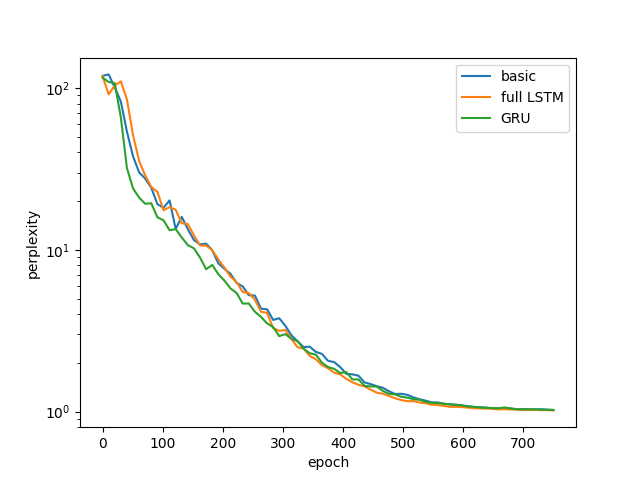
\includegraphics[scale=0.5]{jason.png}
    \caption{S2VT 結果}
    \label{fig:jason}
   \endminipage \hfill
    \minipage{0.5\textwidth}
    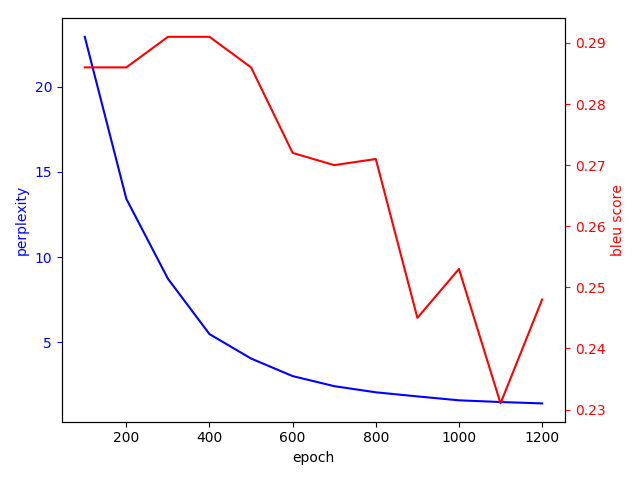
\includegraphics[scale=0.5]{score.png}
    \caption{preplexity 與 score 的關聯}
    \label{fig:score}
   \endminipage
  \end{figure}

\section{Team division}
\begin{table}[h]
\centering
\begin{tabular}{ |C{2cm}|C{10cm}| }
  \hline
  孫凡耕 & Seq2Seq、分配組內工作、教導組員\\
  \hline
  羅啟心 & Tensorboard、Experiment\\
  \hline
  郭子生 & S2VT、Experiment\\
  \hline
  許晉嘉 & 統整撰寫報告、跑實驗、優化 word embedding\\
  \hline
\end{tabular}
\end{table}
% End of Team division

\end{document}
